\documentclass[11pt]{article}
\usepackage{graphicx}
\usepackage{listings}
\usepackage{anysize}
\usepackage{comment}
\usepackage{float}
\renewcommand{\topfraction}{0.9}    % max fraction of floats at top
\renewcommand{\bottomfraction}{0.8}
\marginsize{2cm}{2cm}{1cm}{2cm}
\lstset{
  language=C,                     % choose the language of the code
}
\begin{document}

\title{Algorithms Coursework}
\author{Xueqi Chen and Haixiao Su}

\maketitle
\section*{Randomised Algorithms}
The below figures indicates the changes in time/number of executions in proportional to the size of the words added into the set for three different randomised algorithms: Skip List, Bloom Filter and Randomised BST. The observed trend for time complexity for Skip List and Bloom Filter all follows the similar pattern, which is predicted to be O(log n).
By running analyse a large amount of times, the graph will demonstrate how the implemented algorithm is performing. The size of set is set to be 5000, and the operation is repeated 500 times to ensure accuracy. As the overall system performance may affect the eventual outcome of the graph, the more time that the test is run, the clearer the graph displays the trend. 
\section*{Add}
\begin{figure}[H]
\begin{minipage}{.5\linewidth}
\centering
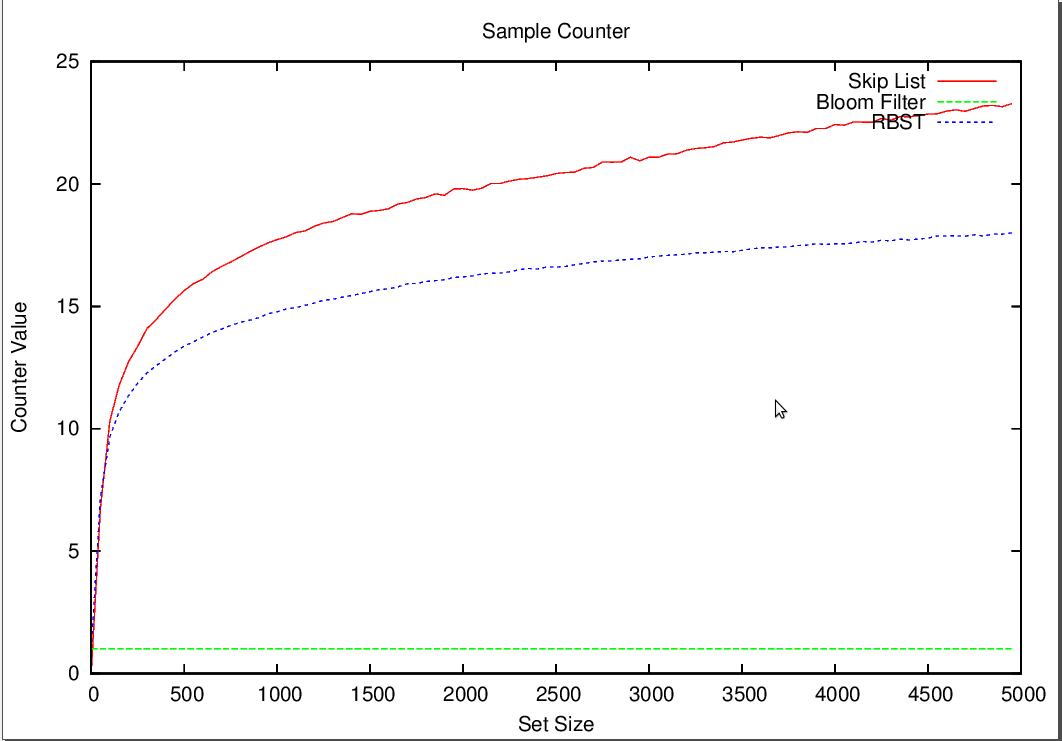
\includegraphics[width=1\linewidth]{addcounter.png}
\caption{addcounter}
\end{minipage}
\hspace{0.5cm}
\begin{minipage}{.5\linewidth}
\centering
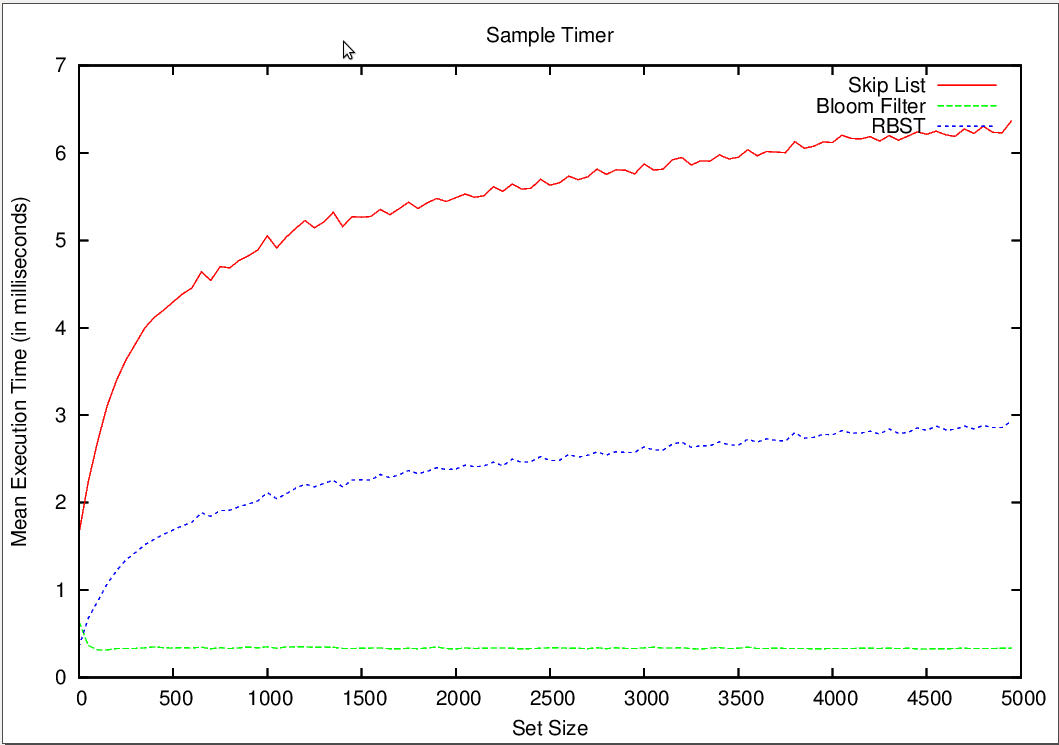
\includegraphics[width=1\linewidth]{addtimer.png}
\caption{addtimer}
\end{minipage}
\end{figure}
\subsection*{Skip List}
Skip List's add function uses randomization generate new j-link element then search to find a position for the new element and link it in as we move down to each level. The time complexity as shown in figure 2, is proportional to the size of the skip list and is bounded by the height of the skip list so thus O(log n). In other words, as there is more words added into the list, the time it takes to add each word becomes relatively less.
\subsection*{Bloom Filter}
Bloom Filter uses two hash functions to determine where a key should be stored in a certain bit of a pocket. No matter how big the size grows, the time complexity would not be affected since it does not involve searching for right position but mathematical calculations. A complicated mathematical calculation (hash function) is not required, as the important pre-requisite requires that all the element inserted to have an unique value to avoid the case of false positive or false negative. Thus the insertion time will be constant as the time it takes to calculate the index is the same no matter what key it is. 
\subsection*{RBST}
RBST randomly alternates between tail insert algorithm and root insert algorithm. This is that the resulting tree could be more balanced, as if the input is ordered, or nearly ordered, the resulting tree would have a complexity for insert and search at O(n). There are two methods we could have used to prevent this: To randomise the input sequence or alternate between two insert methods. The second one was chosen as it is impossible to randomise the input sequence if the input is unknown at the start of the procedure. The complexity is demonstrated to be O(log n), but to be much lower than that of the Skip List. This is because inserting elements into Skip List requires links to be made over several levels, whereas the one single link is established with the new element inserted into RBST. The similar shape for the RBST and Skip List graph indicates that both data structure has similar storage methods, therefore will have similar relativity when inserting an element. 

\section{Delete}
\begin{figure}[H]
\begin{minipage}{.5\linewidth}
\centering
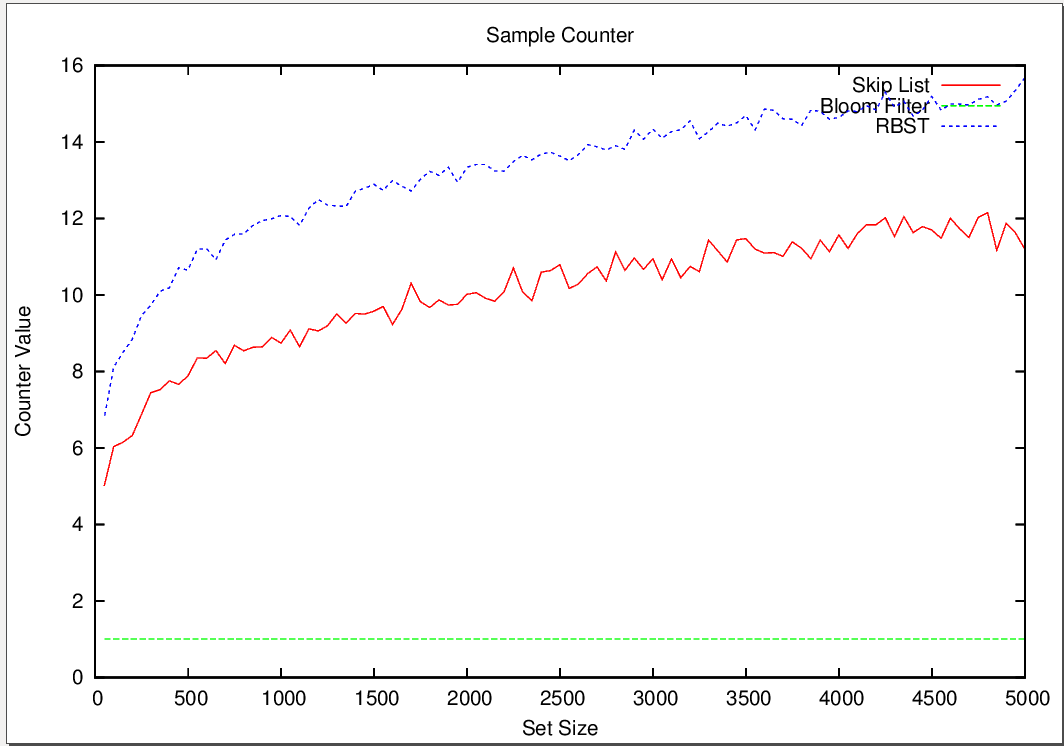
\includegraphics[width=1\linewidth]{delcounter.png}
\caption{delcounter}
\end{minipage}
\hspace{0.5cm}
\begin{minipage}{.5\linewidth}
\centering
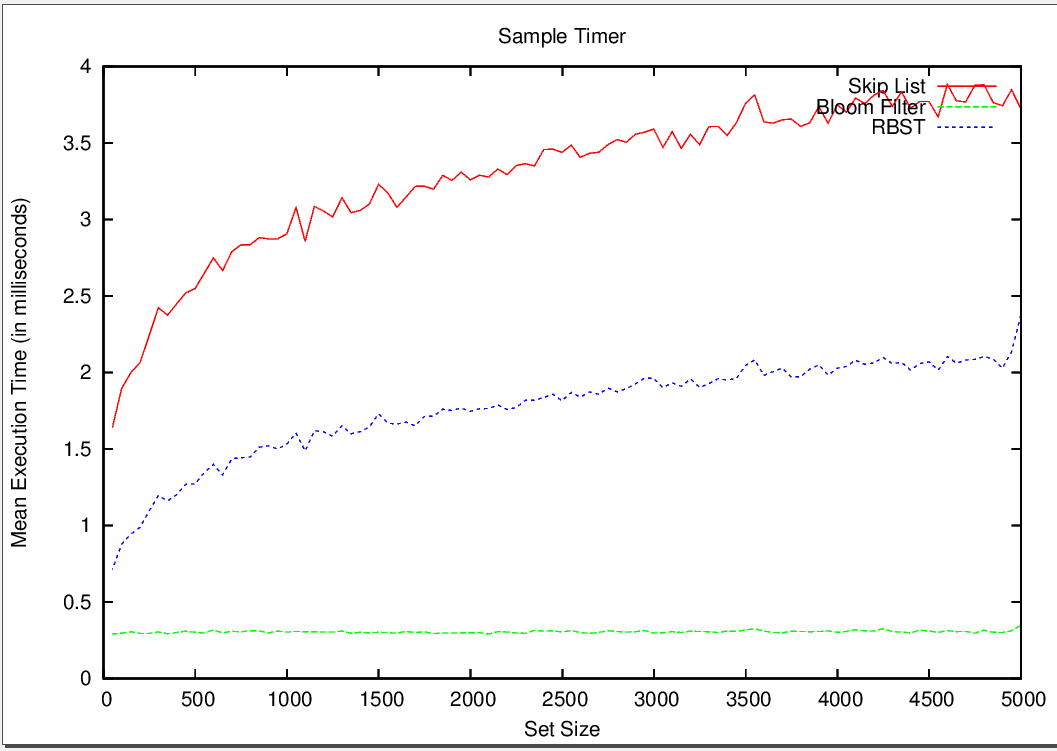
\includegraphics[width=1\linewidth]{deltimer.png}
\caption{deltimer}
\end{minipage}
\end{figure}
\subsection*{Skip List}

\subsection*{Bloom Filter}
The complexity for the Bloom Filter is constant, as the algorithm only requires to change the relevant bits of the Bit Vector to zero. The time for this operation is same for all strings, as the functions that operates on them is the same. However, a clash may occur, as if 3 of the elements shared bits, then deleting one element will affect the outcome of the others. This can be avoided with a better hash function. 
\subsection*{RBST}
The counter value for the RBST is higher than that of the the Skip List even though the execution time is the other way around. This indicate that the number of the times that delete function is called on RBST is higher than that of the Skip List. This is understandable, as the number of times it takes to get to the actual element is similar, however, the deletion process requires more work for the Skip List. E.g. with deletion and replacing the links between the nodes, whereas with RBST, only two relink is required. The number of times it takes to call on the RBST del function is more as I HAVE NO IDEA NEED TO ASK TOMORROW!!!
\section{Find}
\begin{figure}[H]
\begin{minipage}{.5\linewidth}
\centering
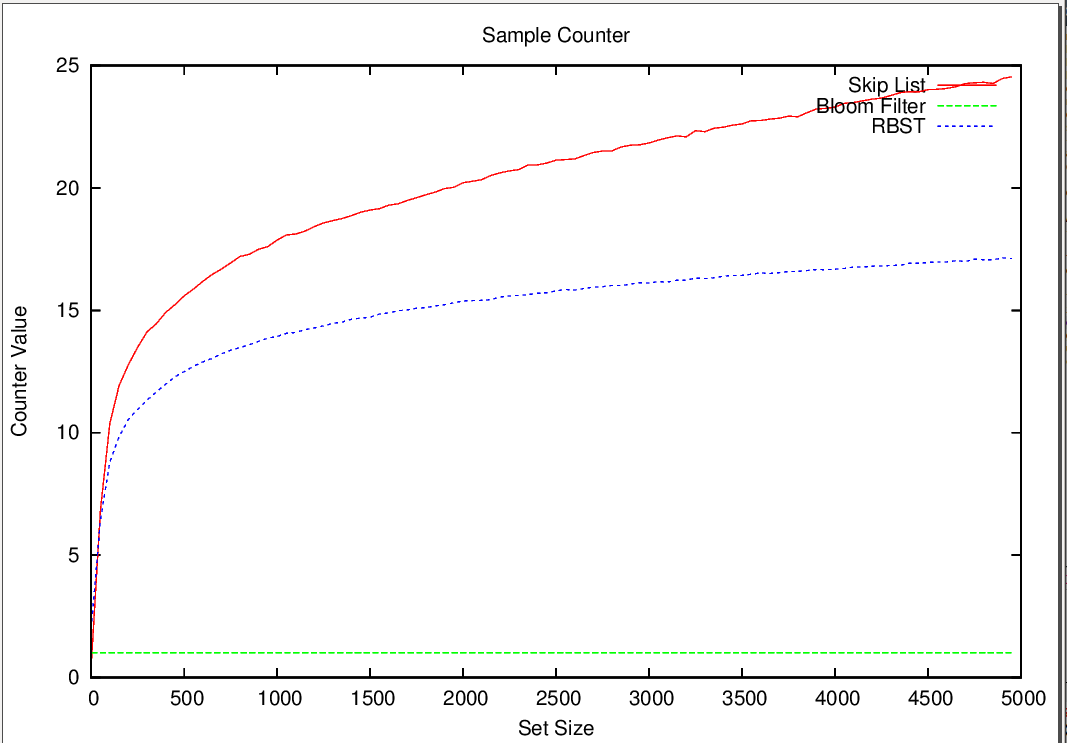
\includegraphics[width=1\linewidth]{findcounter.png}
\caption{findcounter}
\end{minipage}
\hspace{0.5cm}
\begin{minipage}{.5\linewidth}
\centering
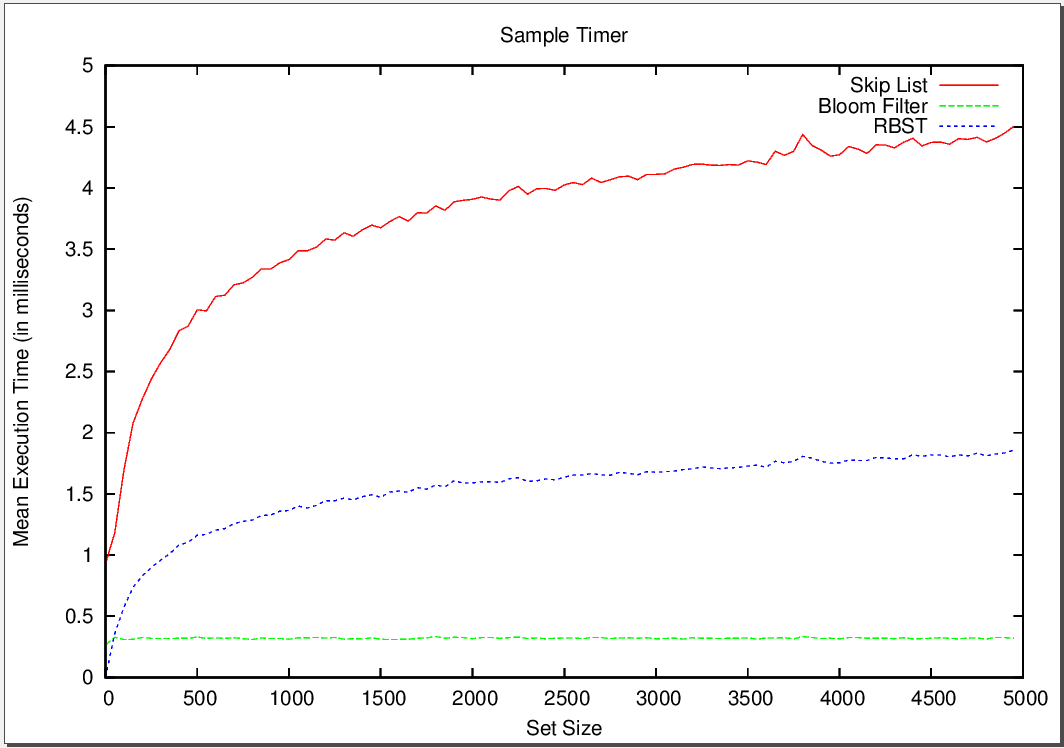
\includegraphics[width=1\linewidth]{findtimer.png}
\caption{findtimer}
\end{minipage}
\end{figure}
\subsection*{Skip List}
\subsection*{Bloom Filter}
The complexity for the Bloom Filter is again constant, as the data structure  only requires the comparison of both indexes to be 1. The mean execution time therefore would be constant. The case of false negative may occur as a result. For example if A requires index 1 and 2, B requires index 3 and 4, C requires index 1 and 3,  then if A and B are in the Bloom Filter and C is not, but C would shown that it is indeed in the Bloom Filter. However, this occurs rarely due to the hash functions that have chosen. 
\subsection*{RBST}
The complexity for the RBST is O(log n). Due to the random add method that have chosen, the RBST would be a balanced one. The worst case scenario would be even less likely to appears. The worst case scenario is still that of the most unbalanced tree, which would literally be a linked list. For the find case, all the algorithm does is that it goes through the children of the tree until the key is found, or returns NULL if the key does not exist in the tree. \\
\end{document}